\documentclass[answers]{exam}
\renewcommand{\solutiontitle}{\noindent\textbf{}\par\noindent}

\usepackage{fullpage} % Package to use full page
\usepackage{parskip} % Package to tweak paragraph skipping
\usepackage{tikz} % Package for drawing
\usepackage{amsmath}
\usepackage{blindtext}
%\usepackage{hyperref}
\usepackage{graphicx}
\usepackage{enumerate}
\usepackage{caption}
\usepackage{subcaption}
\usepackage{multicol}
\usepackage{mathptmx}
\usepackage{amsmath}
\usepackage{amssymb}
\usepackage{nameref}
\usepackage{minted}
\usepackage{graphicx}
\usepackage{hyperref}
\hypersetup{
    colorlinks=true,
    linkcolor=blue,
    filecolor=magenta,      
    urlcolor=blue,
}

\newcommand{\mypoints}[1]{\textcolor{red}{(#1 points)}}
\newcommand{\achuta}[1]{\textcolor{magenta}{Achuta: #1}}
\newcommand{\myinput}[1]{\textcolor{blue}{#1}}

\title{\normalfont \normalsize
\textsc{{Department of ECE, UCLA \\
ECE 188: Computer Vision}}
\date{\vspace{-12ex}}
}
\begin{document}
\maketitle
\rule{\linewidth}{0.8pt} \\[6pt] 
\noindent
\large\textbf{\textsc{Instructor:}} Prof. Achuta Kadambi, Prof. Stefano Soatto \hfill \large\textbf{\textsc{Name:}} \myinput{Anuj Agrawal}\\
\large\textbf{\textsc{TA:}} Zhen Wang \hfill 
\large\textbf{\textsc{UID:}} \myinput{605627630}
\rule{\linewidth}{0.8pt} \\[6pt] 

\begin{center}
{\textsc{Homework 4}} 
\end{center}
% \vspace{2cm}


\begin{table}[h]
\centering
\resizebox{0.8\textwidth}{!}{%
\begin{tabular}{cccc}
\hline
\multicolumn{1}{c}{\textsc{Problem}} &
\multicolumn{1}{c}{\textsc{Type}} &
\multicolumn{1}{c}{\textsc{Topic}} & \multicolumn{1}{c}{\textsc{Max. Points}} \\  \hline \\ 
  1 & Analytical & Machine Learning Basics &  10 \\ [2mm]
 2 & Coding & Training a Classifier &  15 \\ [2mm]
 3 & Interview Questions (Bonus) & Miscellaneous &  15 \\  [2mm]
 4 & Analytical & Generative adversarial networks  &  5 \\  [2mm]
%  [2mm]
    \hline
\end{tabular}
}
\caption*{}
\label{}
\end{table}
\section*{Motivation}
The problem set gives you a basic exposure to machine learning approaches and techniques used for computer vision tasks such as image classification. You will train a simple classifier network on CIFAR-10 dataset using \href{https://colab.research.google.com/notebooks/intro.ipynb#recent=true}{google colab}. We have provided pytorch code for the classification question, you are free to use any other framework if that's more comfortable.  

The problem set consists of two types of problems: 
\begin{itemize}
    \item analytical questions to solidify the concepts covered in the class, and
    \item coding questions to provide a basic exposure to building a machine learning classifier using pytorch.
\end{itemize}

\emph{This problem set also exposes you to a variety of machine learning questions commonly asked in job/internship interviews}


\section*{Homework Layout}
The homework consists of 3 problems in total, with subparts for each problem. There are 2 types of problems in this homework - analytical and coding. All the problems need to be answered in the Overleaf document. Make a copy of the Overleaf project, and fill in your answers for the questions in the solution boxes provided. 

For the analytical questions you will be directly writing their answers in the space provided below the questions. For the coding problems you need to use the Jupyter notebooks (see the Jupyter notebook for each sub-part which involves coding). You are provided with 1 jupyter notebook for Problem 2. After writing your code in the Jupyter notebook you need to copy paste the same code in the space provided below that question on Overleaf. In some questions you are also required to copy the saved images (from Jupyter) into the solution boxes in Overleaf. For the classification question, upload the provided notebook to google colab, and change the runtime type to GPU for training the classifier on GPU. Refer to question 2 for more instructions/details. 

\section*{Submission}

You will need to make two submissions: (1) Gradescope: You will submit the Overleaf PDF with all the answers on Gradescope. (2) CCLE: You will submit your Jupyter notebooks (.ipynb file) with all the cells executed on CCLE. 

\section*{Software Installation}

You will need Jupyter to solve the homework. 
You may find these links helpful: 
\begin{itemize}
    \item Jupyter (https://jupyter.org/install)
    \item Anaconda (https://docs.anaconda.com/anaconda/install/)
\end{itemize}

\newpage


\newpage
\section{Machine Learning Basics \mypoints{10}}
\subsection{Calculating gradients \mypoints{2.0}}
A major aspect of neural network training is identifying optimal values for all the network parameters (weights and biases). Computing gradients of the loss function w.r.t these parameters is an essential operation in this regard (gradient descent). For some parameter $w$ (a scalar weight at some layer of the network), and for a loss function $L$, the weight update is given by $w:=w-\alpha\frac{\partial L}{\partial w}$, where $\alpha$ is the learning rate/step size.

Consider (a) $w$, a scalar, (b) $\mathbf{x}$, a vector of size $(m\times 1)$, (c) $\mathbf{y}$, a vector of size $(n\times 1)$ and (d) $\mathbf{A}$, a matrix of size $(m\times n)$. Find the following gradients, and express them in the simplest possible form (boldface lowercase letters represent vectors, boldface uppercase letters represent matrices, plain lowercase letters represent scalars):
\begin{itemize}
    \item $z=\mathbf{x}^{T}\mathbf{x}$, find $\frac{dz}{d\mathbf{x}}$
    \item $z=Trace(\mathbf{A}^{T}\mathbf{A})$, find $\frac{dz}{d\mathbf{A}}$
    \item $z=\mathbf{x}^{T}\mathbf{A}\mathbf{y}$, find $\frac{\partial z}{\partial\mathbf{y}}$
    \item $\mathbf{z}=\mathbf{A}\mathbf{y}$, find $\frac{d\mathbf{z}}{d\mathbf{y}}$
\end{itemize}

You may use the following formulae for reference:
\begin{equation*}
    \frac{\partial z}{\partial \mathbf{x}}
    =
    \begin{bmatrix}
        \frac{\partial z}{\partial x_{1}}\\
        \frac{\partial z}{\partial x_{2}}\\
        \vdots\\
        \frac{\partial z}{\partial x_{m}}
    \end{bmatrix}
    ,
    \frac{\partial z}{\partial \mathbf{A}}
    =
    \begin{bmatrix}
        \frac{\partial z}{\partial A_{11}} & \frac{\partial z}{\partial A_{12}} & \dots  & \frac{\partial z}{\partial A_{1n}} \\
        \frac{\partial z}{\partial A_{21}} & \frac{\partial z}{\partial A_{22}} & \dots  & \frac{\partial z}{\partial A_{2n}} \\
        \vdots & \vdots & \ddots & \vdots \\
        \frac{\partial z}{\partial A_{m1}} & \frac{\partial z}{\partial A_{m2}} & \dots  & \frac{\partial z}{\partial A_{mn}}
    \end{bmatrix}
    ,
    \frac{\partial \mathbf{y}}{\partial \mathbf{x}}
    =
    \begin{bmatrix}
        \frac{\partial y_{1}}{\partial x_{1}} & \frac{\partial y_{2}}{\partial x_{1}} & \dots  & \frac{\partial y_{n}}{\partial x_{1}} \\
        \frac{\partial y_{1}}{\partial x_{2}} & \frac{\partial y_{2}}{\partial x_{2}} & \dots  & \frac{\partial y_{n}}{\partial x_{2}} \\
        \vdots & \vdots & \ddots & \vdots \\
        \frac{\partial y_{1}}{\partial x_{m}} & \frac{\partial y_{2}}{\partial x_{m}} & \dots  & \frac{\partial y_{n}}{\partial x_{m}}
    \end{bmatrix}
\end{equation*}
\begin{solution}
1. $z=\mathbf{x}^{T}\mathbf{x}$, $\frac{dz}{d\mathbf{x}} = 2\mathbf{x}$\\
2. $z=Trace(\mathbf{A}^{T}\mathbf{A})$, $\frac{dz}{d\mathbf{A}} = 2\mathbf{A} $\\
3. $z=\mathbf{x}^{T}\mathbf{A}\mathbf{y}$, $\frac{\partial z}{\partial\mathbf{y}} = \mathbf{x}^{T}\mathbf{A}$, since the result should be a $(m \times 1)$ so we transpose, s.t., $\frac{\partial z}{\partial\mathbf{y}} = (\mathbf{x}^{T}\mathbf{A})^{T} = \mathbf{A}^{T}\mathbf{x}$\\
4. $\mathbf{z}=\mathbf{A}\mathbf{y}$, $\frac{d\mathbf{z}}{d\mathbf{y}} = \mathbf{A}$
\end{solution}

\subsection{Deriving Cross entropy Loss \mypoints{6.0}}
In this problem, we derive the cross entropy loss for binary classification tasks. Let $\hat{y}$ be the output of a classifier for a given input $x$. $y$ denotes the true label (0 or 1) for the input $x$. Since $y$ has only 2 possible values, we can assume it follow a Bernoulli distribution w.r.t the input $x$. We hence wish to come up with a loss function $L(y, \hat{y})$, which we would like to minimize so that the difference between $\hat{y}$ and $y$ reduces. A Bernoulli random variable (refresh your pre-test material) takes a value of 1 with a probability $k$, and 0 with a probability of $1-k$.  

(i) Write an expression for $p(y|x)$, which is the probability that the classifier produces an observation $\hat{y}$ for a given input. Your answer would be in terms of $y, \hat{y}$. Justify your answer briefly. 
\begin{solution}
$p(y|x) = 
     \begin{cases}
       \text{k,} &\quad\text{if y = 1}\\
       \text{1-k,} &\quad\text{if y = 0} \\
     \end{cases}\\
     \\$
$p(y|x) = (k)^y(1-k)^{1-y}$

Since the output of the classifier for a given input is given by $\hat{y}$,\\
$p(y|x) = (\hat{y})^y(1-\hat{y})^{1-y}$
\end{solution}
(ii) Using (i), write an expression for $\log p(y|x)$. $\log p(y|x)$ denotes the log-likelihood, which should be maximized.
\begin{solution}
$log p(y|x) = y log(\hat{y}) + (1-y)log(1-\hat{y})$
\end{solution}
(iii) How do we obtain $L(y, \hat{y})$ from $\log p(y|x)$? Note that $L(y, \hat{y})$ is to be minimized 
\begin{solution}
$L(y, \hat{y}) = - log p(y|x)$\\
$L(y, \hat{y}) = - y log(\hat{y}) - (1-y)log(1-\hat{y})$
\end{solution}

\subsection{ Perfect Classifier (?) \mypoints{2.0}}

You train a classifier on a training set, achieving an impressive accuracy of 100 \%. However to your disappointment, you obtain a test set accuracy of 20 \%.  For each suggestion below, explain why (or why not) if these suggestions may help improve the testing accuracy.
\begin{enumerate}
    \item Use more training data
    \item Add L2 regularization to your model
    \item Increase your model size, i.e. increase the number of parameters in your model
    \item Create a validation set by partitioning your training data. Use the model with highest accuracy on the validation set, not the training set. 
\end{enumerate}

\begin{solution}
1. Using more training data with prevent the model from over-fitting as it will induce randomness to the training process. This might help the model to improve accuracy over the test dataset as the model is more generalized over the training dataset.\\
\\
2. Regularization of our model prevent the over-fitting of the model by penalizing complex models,i.e., rather than just minimizing the loss we all minimize the complexity ($L_2$ regularization term) of the model. By penalizing our weights in the configuration we balance them. This will lead to a model that is less accurate during training but in turn prevents over-fitting. $L_2$ regularization term is the sum of square weights,i.e., it penalises large weights which in turn give more generalizes training.\\
\\
3. The need to increase the model size depends case by case. If the model is small such that it is not able to comprehensively understand the features and classes in a given dataset then increasing the model size will be a beneficial as a better representation of the dataset. Whereas if the model is already large enough or the dataset is very small in comparison then there is a high chance that the model memorizes the entire training dataset and not just relevant features leading to over-fitting. Increasing the size of model in turn will further decrease the performance from a general solution.\\
\\
4. Creating a validation set will help increase accuracy of the solution as it outputs the inference results of the model on a dataset not previously seem by the model which is close to the real time input to the model. This will optimize the solution to a more general solution. A higher accuracy on the validation set in general indicates a higher accuracy on model inference.


\end{solution}


\newpage

\section{Implementing an image classifier using PyTorch \mypoints{15.0}}
In this problem you will implement a CNN based image classifier in pytorch. We will work with the CIFAR-10 dataset. Follow the instructions in jupyter-notebook to complete the missing parts. For this part, you will use the notebook named PSET4\_Classification. For training the model on colab gpus, upload the notebook on google colab, and change the runtime type to GPU. 

\subsection{Loading Data \mypoints{2.0}}
(i) Explain the function of transforms.Normalize() function (See the Jupyter notebook Q1 cell). How will you modify the arguments of this function for gray scale images instead of RGB images. \\
(ii) Write the code snippets to print the number of training and test samples loaded. 

Make sure that your answer is within the bounding box.
\begin{solution}
(i) transform.Normalize() function is used to normalize the dataset from [0, 1] to [-1, 1]. The function inputs 3 values corresponding to the mean and 3 values corresponding to the standard deviation for the 3 channels (RGB). The function works by normalizing the value of each channel in the image using the formula,\\
\textbf{Image = (Image - Mean)/ Std}\\
In case, it is a greyscale image we modify the output as:\\
\textbf{transforms.Normalize((0.5, ), (0.5, ))}\\

(ii)
% Paste your code within the block
\begin{minted}{python}
print(len(train_data))
print(len(test_data))
\end{minted}
\end{solution}

\subsection{Classifier Architecture \mypoints{6.0}}
(See the Jupyter Notebook) Please  go  through  the  supplied  code  that defines the architecture (cell Q2 in the Jupyter Notebook), and answer the following questions. 

\begin{enumerate}
\item Describe the entire architecture. The description for each layer should include details about kernel sizes, number of channels,  activation functions and the type of the layer. 

\item What does the padding parameter control?

\item Briefly explain the max pool layer.

\item What would happen if you change the kernel size to 3 for the CNN layers without changing anything else? Are you able to pass a test input through the network and get back an output of the same size? Why/why not? If not, what would you have to change to make it work?

\item While backpropagating through this network, for which layer you don't need to compute any additional gradients? Explain Briefly Why. 
\end{enumerate}

\begin{solution}
1. 
The entire architecture includes 2 2D convolution layers with max pooling layer after each convolution of operation. The output of the max pooling layer is flattened and passed to 3 fully connected layers.\\
\textbf{Layer 1}: This layer inputs a normalized image (mean: (0.5, 0.5, 0.5) and std: (0.5, 0.5,0.5)) with 3 channels corresponding to the RGB. The convolution layer output 6 channel. \\
Total number of convolution operations:  6*3 = 18.\\
Kernel size, K : 5 X 5\\
Stride, S: 1\\
Padding, P: 0\\
Output size: [(W−K+2P)/S]+1 = [(32 - 5 +2*0)/1] + 1 = 28, (28 X 28 X 6)\\
Activation function: Relu\\
\\
\textbf{Layer 2}: This layer input the 28 X 28 X 6 input tensor and performs a max pooling operation with kernel size 2 X 2 such that it reduced every 2 X 2 region to a single pixel with value corresponding to the maximum value in the region.\\
Kernel size, K : 2 X 2\\
Stride, S: 2\\
Output size: 14 X 14 X 6\\
\\
\textbf{Layer 3}: This layer inputs a tensor of dimension of size 14 X 14 X 6. The convolution layer output 6 channel.\\ 
Total number of convolution operations:  6*16 = 96.\\
Kernel size, K : 5 X 5\\
Stride, S: 1\\
Padding, P: 0\\
Output size: [(W−K+2P)/S]+1 = [(14 - 5 +2*0)/1] + 1 = 10, (10 X 10 X 16)\\
Activation function: Relu\\
\\
\textbf{Layer 4}: This layer input the 10 X 10 X 16 input tensor and performs a max pooling operation with kernel size 2 X 2 such that it reduced every 2 X 2 region to a single pixel with value corresponding to the maximum value in the region.\\
Kernel size, K : 2 X 2\\
Stride, S: 2\\
Output size: 5 X 5 X 16\\
\\
We flatten out the output of this layer into a single 400 dimension feature vector .\\
\\
\textbf{Layer 5}: This layer is a fully connected layer with input dimension vector of size 400.\\
Output size : 120\\
Total number of weights: 400 X 120 = 48,000\\
Total number of biases: 120\\
\\
\textbf{Layer 6}: This layer is a fully connected layer with input dimension vector of size 120.\\
Output size : 84\\
Total number of weights: 120 X 84 = 10080\\
Total number of biases: 84\\
\\
\textbf{Layer 7}: This layer is a fully connected layer with input dimension vector of 84.\\
Output size : 10\\
Total number of weights: 10 X 84 = 840\\
Total number of biases: 10\\
\\
These 10 dimensional output vector corresponds to the 10 classes. To find the classification output find the argument corresponding to the maximum vector element.\\
\\
2.The padding parameter controls the amount of pixels to be appended around the edges of the images such that the output of the convolution operation is of a defined size. Default is zero padding. Without padding the output will be of smaller size then the input.\\
\\
3. Max pooling layer for a given kernel size output the maximum pixel value amongst all the pixels overlapping the kernel. It is a non linear operation that is used to decrease the dimensionality of the input tensor in order to train over the essential abstract input data and prevent over-fitting. It in turn reduces the number of parameters of the model. This operation also helps make the model invariant to change in pixel position as maximum value within a kernel remains same irrespective of order.\\
\\
4. Changing the kernel size to 3 for the CNN layers won't pass the test case and get an output of the same size as with no padding the output of the conv2d size layer depends on the kernel size. Such that, the output of the 2nd max pooling layer will be 16 X 6 X 6 instead of 16 X 5 X 5. This is because both convolution layers have different output with respect to the input size( 30 X 30 and 13 X 13 for 1st and 2nd convolution respectively).
To make the model work, we can make the following changes:\\
1) self.fc1 = nn.Linear(16 * 6 * 6, 120)\\
2) x = x.view(-1, 16 * 6 * 6)\\
\\
5. While backpropagating we do not need to compute any gradient for the \textbf{flatten} or \textbf{max pooling} layer as these layers do not have training parameters associated with them.
\end{solution}

\subsection{Training the network \mypoints{3.0}}

(i) (See the Jupyter notebook.) Complete the code in the jupyter notebook for training the network on a CPU, and paste the code in the notebook. Train your network for 3 epochs. Plot the running loss (in the notebook) w.r.t epochs. 
\begin{solution}
\begin{minted}{python}
### Complete the code in the training box 

## for reproducibility
torch.manual_seed(7)
np.random.seed(7)

## Instantiating classifier
net = Net()

## Defining optimizer and loss function
criterion = nn.CrossEntropyLoss()
optimizer = optim.SGD(net.parameters(), lr=0.001, momentum=0.9)


## Defining Training Parameters

num_epochs = 3 # 2 for CPU training, 10 for GPU training
running_loss_list = [] # list to store running loss in the code below 
for epoch in range(num_epochs):  # loop over the dataset multiple times
    running_loss = 0.0
    for i, data in enumerate(train_loader, 0):
        # get the inputs; data is a list of [inputs, labels]
        inputs, labels = data
        #===============================================#
        optimizer.zero_grad() # zero parameter gradients
        outputs = net(inputs) #forward
        loss = criterion(outputs, labels)
        loss.backward() #backward
        optimizer.step() #optimize
        #===============================================#
        # print statistics
        running_loss += loss.cpu().item()
        if i % 250 == 249:    # print every 250 mini-batches
            print('[{}, {}] loss: {:.3f}'.format(epoch + 1, i + 1, running_loss / 250))
            running_loss_list.append(running_loss)
            running_loss = 0.0
            
print('Training Complete')
PATH = './net.pth'
torch.save(net.state_dict(), PATH)

## complete the code to plot the running loss per 250 mini batches curve

def plot_loss_curve(running_loss_list):
  x_range = np.arange(1, len(running_loss_list)*250, 250)
  plt.xlabel("interation number")
  plt.ylabel("loss")
  plt.title("interation number vs loss ")
  plt.plot(x_range, np.array(running_loss_list))
  plt.show()
\end{minted}

\begin{figure}[H]
    \centering
    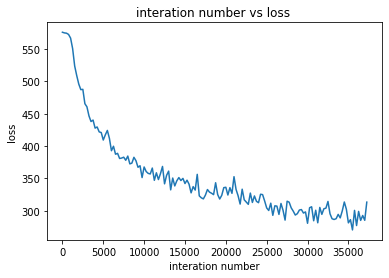
\includegraphics[width=0.9\linewidth]{Images/cpu.png}
\end{figure}
\end{solution}

(ii) (See the Jupyter notebook.) Modify your training code, to train the network on the GPU. Paste here the lines that need to be modified to train the network on google colab GPUs. Train the network for 20 epochs
\begin{solution}
\begin{minted}{python}

net = Net().cuda()
...
        outputs = net(inputs.cuda()) #forward
        loss = criterion(outputs.cuda(), labels.cuda())
...
        running_loss += loss.cuda().item()
...
\end{minted}
\begin{figure}[H]
    \centering
    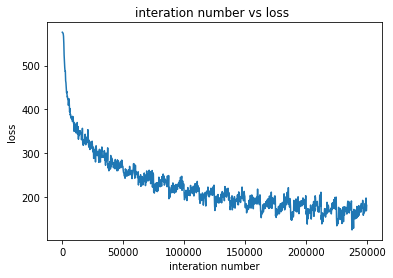
\includegraphics[width=0.9\linewidth]{Images/gpu.png}
\end{figure}
\end{solution}

(iii) Explain why you need to reset the parameter gradients for each pass of the network
\begin{solution}
We reset the gradient parameters using $optimizer.zero\_grad()$ as for each mini-batch we aim to calculate new gradients. If we do not make these parameters zero, then the gradients will accumulate over the entire batch. This will discard the advantage (stochastic properties) of using mini-batches.
\end{solution}
\subsection{Testing the network \mypoints{4.0}}

(i) (See the jupyter-notebook) Complete the code in the jupyter-notebook to test the accuracy of the network on the entire test set. 
\begin{solution}
\begin{minted}{python}
### Accuracy on whole data set
correct = 0
total = 0
with torch.no_grad():
    for data in test_loader:
        images, labels = data
        outputs = net(images)
        _, predicted = torch.max(outputs.data, 1)
        total += labels.size(0)
        correct += (predicted == labels).sum().item()
acc  = 100*correct/total# stores the accuracy computed in the above loop 
print('Accuracy of the network on the 10000 test images: %d %%' % (acc))
\end{minted}
\end{solution}
(ii) Train the network on the GPU with the following configurations, and report the testing accuracies and running loss curves -

\begin{itemize}
    \item Training Batch Size 4, 20 training epochs
    \item Training Batch Size 4, 5 epochs
    \item Training Batch Size 16, 5 epochs
    \item Training Batch Size 16, 20 epochs 
\end{itemize}

\begin{solution}
\\
1. Accuracy of the network on the 10000 test images: 61 \%
\begin{figure}[H]
    \centering
    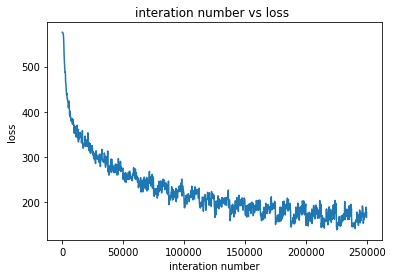
\includegraphics[width=0.9\linewidth]{Images/gpu0.png}
\end{figure}
\\
2. Accuracy of the network on the 10000 test images: 61 \%
\begin{figure}[H]
    \centering
    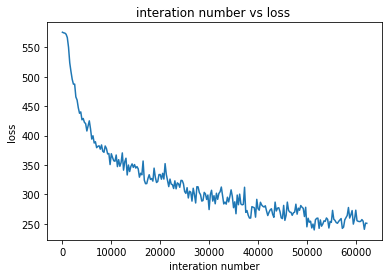
\includegraphics[width=0.9\linewidth]{Images/gpu2.png}
\end{figure}
\\
3. Accuracy of the network on the 10000 test images: 58 \%
\begin{figure}[H]
    \centering
    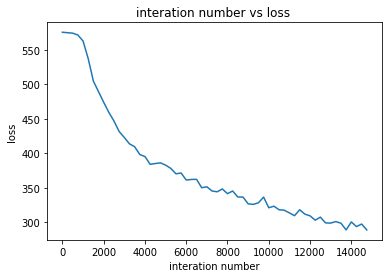
\includegraphics[width=0.9\linewidth]{Images/gpu3.png}
\end{figure}
\\
4. Accuracy of the network on the 10000 test images: 64 \%
\begin{figure}[H]
    \centering
    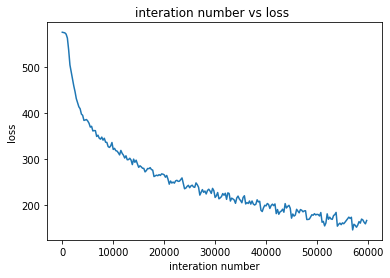
\includegraphics[width=0.9\linewidth]{Images/gpu4.png}
\end{figure}
\end{solution}
(iii) Explain your observations in (ii) 
\begin{solution}
1) Increasing the batch size from 4 to 16 with a smaller epochs number 5 decreases the test accuracy of the model. This is because of the overfitting that occurs when using a bigger batch size.\\
2) Further increasing the number of epochs actually improves the testing accuracy (16 batch size and 20 epoches). This is due to the fact that a larger number of iteration causes the model to actually accumulates a more generalized behavior. Where a larger batch size decreases the testing accuracy as this will induce less noise in the model but since we have a higher number of iterations we compensate for this.\\
3) We benefit by having a larger batch size because since it makes out gradients more accurate at each step and given a sufficient number of iterations will outperform a smaller batch size.
\end{solution}

\section{Interview Questions \mypoints{15}}

\subsection{Batch Normalization \mypoints{4}}
Explain \\ 
(i) Why batch normalization acts as a regularizer. \\ 
(ii) Difference in using batch normalization at training vs inference (testing) time. 
\begin{solution}
1. Batch Normalization acts a regularize because it calculates the mean and std w.r.t each mini-batch it is performing training on. This adds stochastic noise to each layer similar to regularization using dropout and hence making the model more general (prevents overfitting).\\
\\
2. Using batch normalization at training time calculates mean and variance over mini-batches for adding regularization effect. However, using batch normalization at inference won't be a good ideas as the calculated valued will be over input image. This will be extremely biased and will produce inaccurate result. One way of solving this problem is by using batch normalization over the entire training data and using at test time.
\end{solution}

\subsection{CNN filter sizes \mypoints{4}}
Assume a convolution layer in a CNN with parameters $C_{in} = 32$, $C_{out} = 64, k = 3$. If the input to this layer has the parameters $C = 32, H = 64, W = 64$. 

(i) What will be the size of the output of this layer, if there is no padding, and stride = 1  \\
(ii) What should be the padding and stride for the output size to be $C = 64, H = 32, W = 32$ 
\begin{solution}
1. Output size: [(W+2P-D(K-1)-1)/S]+1 = [(64 - 1(3-1) -1 +2*0)/1] + 1 = 62\\
2. Output size: [(W+2P-D(K-1)-1)/S]+1 = 32\\
which gives, Padding = 1 and Stride = 2
\end{solution}

\subsection{L2 regularization and Weight Decay \mypoints{4}}
Assume a loss function of the form $L(y,\hat{y})$ where $y$ is the ground truth and $\hat{y} = f(x,\boldsymbol{w})$. $x$ denotes the input to a neural network (or any differentiable function) $f()$ with paramters/weights denoted by $\boldsymbol{w}$. Adding $L2$ regularization to $L(y, \hat{y})$ we get a new loss function $L'(y, \hat{y}) = L(y, \hat{y}) + \lambda \boldsymbol{w}^{T}\boldsymbol{w}$, where $\lambda$ is a hyperparameter. Briefly explain why $L2$ regularization causes weight decay. Hint: Compare the gradient descent updates to $\boldsymbol{w}$ for $L(y,\hat{y})$ and $L'(y, \hat{y})$. Your answer should fit in the given solution box.
\begin{solution}
L2 regularization causes weight decay because the loss function includes a quadratic weight term along with the loss over output $L(y,\hat{y})$. This term penalizes the accuracy of the model by keeping into account the model complexity and thus preventing over-fitting.
During the backpropagation, the optimizier will take into account the increase in the model complexity as larger weights will cause higher loss. Hence the gradient decent with L2 regularization causes a smaller weight change and hence a a weight delay. 
\end{solution}

\subsection{Why CNNs? \mypoints{3}} 
Give 2 reasons why using CNNs is better than using fully connected networks for image data.
\begin{solution}
1. CNNs allow for the model to preserve the structure information of the input image which a MLP architecture destroys. A CNN model can learn and extract these features/structural information and further pass to a fully connected network for classification.\\
2. CNN uses convolution operation over trained kernel values so it drastically reduces model complexity and size. Where as FCNs has weighted connections from all input layers to output layer.
\end{solution}

\newpage
\section{GAN (Bonus) \mypoints{5.0}}
\subsection{Understanding GANs- Loss function \mypoints{2.0}}
Mathematically express the overall GAN loss function being used. For a (theoretically) optimally trained GAN: (a) what is the ideal behavior of the discriminator, and (b) what is the value of the overall loss function?
\begin{solution}
\vspace{2cm} % remove this
\end{solution}

\subsection{Understanding GANs- Gradients \mypoints{2.0}}
Assume that you are working with a GAN having the following architecture:

Generator: Input: $\mathbf{x}$ shape $(2,1) \rightarrow$ Layer: $\mathbf{W_g}$ shape $(5,2) \rightarrow$ ReLU $\rightarrow$ Output: $\mathbf{y}$ shape $(5,1)$
Discriminator: Input: $\mathbf{z}$ shape $(5,1) \rightarrow$ Layer: $\mathbf{W_d}$ shape $(1,5) \rightarrow$ Sigmoid $\rightarrow$ Output: $b$ shape $(1,1)$

Therefore, the generator output is given by, $\mathbf{y} = ReLU(\mathbf{W_g}\mathbf{x})$, and the discriminator output is given by $b = Sigmoid(\mathbf{W_d}\mathbf{z})$.
Express the gradient of the GAN loss function, with respect to the weight matrices for the generator and discriminator. 


You may use the following information: 
\begin{equation*}
    Sigmoid(x) = \frac{1}{1+e^{-x}}
\end{equation*}
\begin{equation*}
    ReLU(x)=\begin{cases}
			x, & \text{if $x  \geq 0$}\\
            0, & \text{if $x<0$}
		 \end{cases}
\end{equation*}

\textit{Hint: Remember that the input here is a vector, not an image.}

\begin{solution}
\vspace{2cm} % remove this
\end{solution}

\subsection{Understanding GANs- Input distributions \mypoints{1.0}}
While training the GAN, the input is drawn from a normal distribution. Suppose in a hypothetical setting, each time the input is chosen from a different, randomly chosen probability distribution. How would this affect the training of the GAN? Justify your answer mathematically.
\begin{solution}
\vspace{2cm} % remove this
\end{solution}
% \bibliographystyle{plain}
% \bibliography{bibliography.bib}


\end{document}